\documentclass{article}
\usepackage[utf8]{inputenc}
\usepackage{graphicx}

\title{Pre-Production Document for Capstone Project}
\author{Abdullah J. Rowaished}
\date{25 June 2019}

\begin{document}
\maketitle
\section{VR Farming Simulator}
The player will be set into a farming environment and will plant seeds into the ground. He will consult the botany book in order to figure out the correct proportions of fertilizer, soil and water. Various farming tools in the vicinity will be used in unique ways and combinations to achieve this. If the plants weren't taken care of properly and weren't harvested in time the crops quality may be affected. The randomized existence of rain or drought will affect the outcome. Something akin to Minecraft's farm.
\begin{figure}[h] %minecraft
\centering
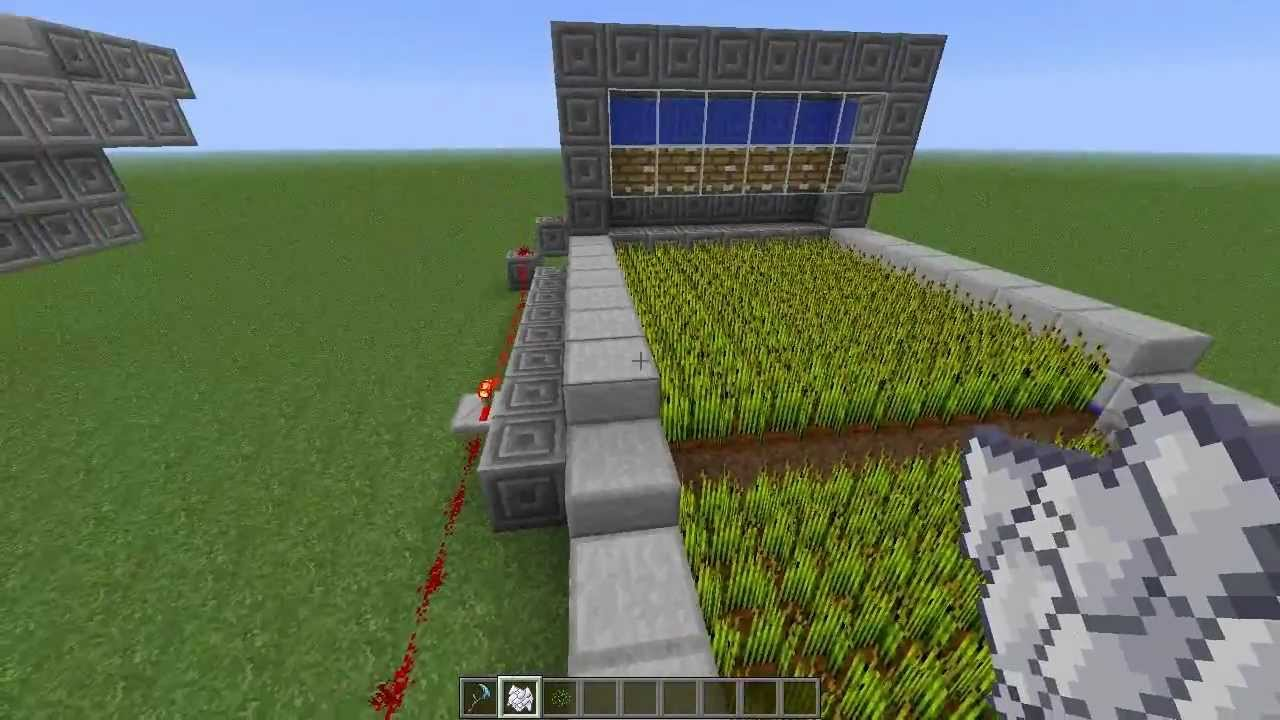
\includegraphics[scale=0.25]{minecraft}
\caption{Farm example in Minecraft}
\end{figure} %minecraft

\section{Features}
\subsection{3D Models}
Using Blender, a set of 3D models shall be created.
\subsubsection{Tools}
A bunch of farming tools will be modeled for players' use via Blender.
\begin{itemize} %Tools
\item \textbf{Scythe}
\item \textbf{Hoe}
\item \textbf{Basket}
\item \textbf{Bucket}
\item \textbf{Spade}
\item \textbf{Watering Pot}
\item \textbf{Animal Trap}
\end{itemize} %Tools
\subsubsection{Produce}
Produce such as fruits and vegetables shall be modeled using Blender also.
\begin{itemize} %Produce
\item \textbf{Apple}, its \textbf{Apple Seed} and \textbf{Apple Tree}
\item \textbf{Pear}, its \textbf{Pear Seed} and \textbf{Pear Tree}
\item \textbf{Orange}, its \textbf{Orange Seed} and \textbf{Orange Tree}
\item \textbf{Wheat}, its \textbf{Grain} and \textbf{Wheat Bushel}
\item \textbf{Melon}, its \textbf{Melon Seed} and \textbf{Melon Growth}
\end{itemize} %Produce
\subsubsection{Environment}
A farm shall be modeled using Blender, alongside its pests.
\begin{itemize} %Environment
\item \textbf{Wooden Fence} sets boundary of the farm
\item \textbf{Soil} Ploughable ground
\item \textbf{Ploughed Soil} Ploughed ground
\item \textbf{Skybox} Atmosphere of the farm
\item \textbf{Hog} Animal acting as pestilence
\end{itemize} %Environment
\subsection{Animations}
\begin{itemize} %Animations
\item \textbf{Hog}
\begin{itemize} %Hog
\item Idle: animal standing by
\item Walking: animal walking towards produce
\item Running: animal running
\item Eating: animal eats crops
\item Trapped: animal getting snared
\end{itemize} %Hog
\item \textbf{Trap} animation for trap closing and opening
\item \textbf{Crops} crops needs to move idly with wind or rain, and harvesting animation
\end{itemize}
\subsection{Sound Effects}
\begin{itemize} %Sound Effects
\item Rain
\item Hog
\item Harvesting
\item Ambiance
\item Music
\item Trap
\end{itemize} %Sound Effects
\section{Game Loop}
\begin{enumerate}
\item Tutorial
\begin{itemize} %Tutorial
\item Welcome to VR Farming Sim. To start, click here.
\item Use Left Joystick to move.
\item Look around to check your environment
\item Pickup any item by holding any Trigger
\item Water the soil
\item Harvest crops with Scythe and Basket
\item Congratulations! You have passed the tutorial!
\end{itemize} %Tutorial
\item Mechanics
\begin{itemize} %Mechanics
\item Player may click "B" to choose how many seasons to 'skip'
\item Goal is to make enough produce to sell and break even or make a profit
\item Resources used to farm deplete with use
\item They can be bought from the market
\item Produce is automatically sold on the market in Harvesting season
\item Rain events are randomized and may give bonuses or penalties per plant
\item Animal raids are also randomized and only incur penalties
\item Rain can be mitigated by predicting weather and under-compensating water
\item Animals can be fought with traps
\item Farm can expand with enough money
\item Player can walk around farm with Left Analog
\item Camera rotation is possible with Right Analog as well as Camera Rig
\end{itemize} %Mechanics
\end{enumerate} %Game Loop
\end{document}